\documentclass[conference]{IEEEtran}
%
% General
%
\usepackage[english]{babel}

%
% Formatting
%
\usepackage{inconsolata}
\usepackage{hyperref}

\usepackage{lettrine}
\usepackage[factor=1700]{microtype}
\newcommand{\subscript}[1]{\text{\kern0.1em#1}}

%
% Figures
%
\usepackage{graphicx}

\setlength{\textfloatsep}{0.5em}

%
% Tables
%
\usepackage{array}
\usepackage{booktabs}
\usepackage{multirow}
\usepackage[flushleft]{threeparttable}

\newcolumntype{L}[1]{>{\raggedright\let\newline\\\arraybackslash\hspace{0pt}}m{#1}}
\newcolumntype{C}[1]{>{\centering\let\newline\\\arraybackslash\hspace{0pt}}m{#1}}
\newcolumntype{R}[1]{>{\raggedleft\let\newline\\\arraybackslash\hspace{0pt}}m{#1}}

\newcolumntype{=}{>{\global\let\currentrowstyle\relax}}
\newcolumntype{-}{>{\currentrowstyle}}

%
% Text shortcuts
%
\renewcommand{\sc}[1]{#1}

\newcommand{\ie}{i.e.}
\newcommand{\eg}{e.g.}

\renewcommand{\tt}[1]{\texttt{#1}}

%
% References
%
\newcommand{\eref}[1]{(\ref{equ:#1})}
\newcommand{\fref}[1]{Fig.~\ref{fig:#1}}
\newcommand{\sref}[1]{Sec.~\ref{sec:#1}}
\newcommand{\tref}[1]{Table~\ref{tab:#1}}

\newcommand{\elab}[1]{\label{equ:#1}}
\newcommand{\flab}[1]{\label{fig:#1}}
\newcommand{\slab}[1]{\label{sec:#1}}
\newcommand{\tlab}[1]{\label{tab:#1}}


\title{
  Fast Synthesis of Power and Temperature\\
  Profiles of Electronic Systems
  \vspace{-1.5em}
}

\author{%Ivan Ukhov, Diana Marculescu, Petru Eles, and Zebo Peng
}

\begin{document}
  \maketitle

  \begin{abstract}
    We present a software framework for a rapid generation of realistic power and
temperature traces of multiprocessor systems. The target audience of the
framework is research studies that leverage learning techniques in order to
achieve their goals such as those developing power- and temperature-aware
management strategies. In this context, the availability of sufficient large
amounts of data---which are essential for learning and, hence, exploration of
research ideas---is rather elusive, to say the least. The presented framework
aims to fulfill this need, that is, to provide profuse representative data to
learn from. The overarching goal is to enable new and facilitate existing
studies by making it feasible to explore novel or revived, highly promising, but
data-demanding techniques for data analysis and prediction such as artificial
neural networks with deep architectures.

  \end{abstract}

  \begin{IEEEkeywords}
    Electronic system,
    machine learning,
    power,
    simulation,
    synthesis,
    temperature,
    traffic,
    workload.
  \end{IEEEkeywords}

  \bstctlcite{IEEEexample:BSTcontrol}

  \section{Introduction} \slab{introduction}
  \lettrine[findent=0.4em, nindent=0em]{\textbf{P}}{ower} consumption and heat
dissipation are of paramount importance. The two inseparable phenomena dictate
limitations on the usage of electronic devices and magnify the costs pertaining
to the deployment and maintenance of electronic systems. Power is essentially
energy, and energy translates willingly to hours of battery life and zeros in
electricity bills. Temperature, on the other hand, is one of the major causes of
permanent damage \cite{jedec}, which necessitates the deployment of adequate
cooling equipments, escalating the overall expenses \cite{chaudhry2015}. The
situation is deteriorated even further by the power-temperature interplay:
higher power leads to higher temperature, and higher temperature strikes back by
making devices consume even more power \cite{liu2007}. Under these
circumstances, it is no surprise that power and temperature have steadily been
in the research limelight and have no plans on leaving this spot.

In this paper, we set out to assist researchers working with power and
temperature in one specific but rather broad context. More concretely, we would
like to facilitate the development of on-chip, data-driven, power- and
temperature-aware solutions for multiprocessor systems. Let us clarify the terms
involved in the previous statement; the approach itself will be described
shortly after. \emph{On-chip} refers to taking decisions online or,
equivalently, at runtime, which is in contrast to having decisions taken
offline, at design time. \emph{Data-driven} refers to the usage of machine
learning \cite{bishop2006}, that is, to the usage of algorithms that learn from
data as opposed to algorithms of any other kind. \emph{Power-aware} refers to
decision-making that takes into account the impact on and the impact of power
(and energy) consumption. Similarly, \emph{temperature-aware} refers to
considering heat dissipation when taking decisions.

We approach the outlined objective by developing a methodology for a fast
synthesis of realistic power and temperature profiles. Our motivation for doing
so is described in the next section, \sref{motivation}, and here we only would
like to remark that data-driven techniques obviously require data to learn from,
and these data might not be easily accessible to researchers for a variety of
reasons, preventing research ideas from flowing freely. The goal of this work is
to eliminate this obstacle.

It is important to realize right from the start that, while artificial data
enable thoughts and ideas to evolve and ripen, the solution being developed will
eventually have to face real data. Therefore, the solution should be tested and,
if needed, calibrated in a stage environment prior to the deployment to a
production environment, which could also be done periodically at the end of a
large development cycle. The usage of synthetic data substantially speeds up the
development process due to the flexibility and fast feedback enabled by such
data, which, in particular, means that one can filter out bad ideas at early
stages and focus solely on the ones which are viable.

The remainder of the paper is organized as follows. The motivation for embarking
on this line of research is given in \sref{motivation}.
Section~\ref{sec:prior-work} provides an overview of the prior work. In
\sref{present-work}, the contributions of the present work are summarized. The
addressed problem is formalized in \sref{problem-formulation}. The proposed
methodology and the corresponding toolchain are described in \sref{methodology}
and \sref{toolchain}, respectively. The usage of our technique is discussed in
\sref{guidelines}. Section \ref{sec:conclusion} concludes the paper.


  \section{Motivation} \slab{motivation}
  \subsection{Power and Temperature}
Accounting for power and temperature is key to achieving effectiveness,
efficiency, and robustness. However, power consumption and heat dissipation are
a result of a myriad of interactions between numerous hardware and software
components comprising modern electronic systems. It is, therefore, difficult to
describe mathematically or algorithmically the impact of a parameter on the
power and temperature characteristics of the system being developed. Moreover,
many aspects of the system are inherently uncertain to the designer. One of the
reasons is process variation \cite{chandrakasan2000}: the properties of
fabricated dies deviate from the nominal ones since process parameters cannot be
controlled precisely using the technologies currently employed in the
fabrication process. Another reason is aging \cite{coskun2006}: the performance
of a system degrades over time due to natural or accelerated wear, which is
unlikely to be uniform. Yet another and perhaps the most consequential reason is
workload: the demand on a system in the field is rarely, if ever, known in the
lab. Such uncertainties inevitably make power and temperature characteristics of
electronic systems uncertain as well.

The above concerns are particularly hard to address from a theoretical
standpoint. They can be better dealt with taking a more pragmatic approach,
namely, making use of on-chip\footnote{In this paper, we use \emph{on-chip},
\emph{online}, and \emph{runtime} interchangeably.} data. To elaborate, assuming
that the system at hand provides basic mechanisms for profiling and monitoring
such as hardware performance counters and thermal sensors, which is typically
the case, direct or indirect power and temperature readings are an invaluable
source of information for making power- and temperature-aware decisions. The
attractiveness of the on-chip-data route is due to the fact that only one
particular fabricated hardware in one particular environment needs to be
considered. More importantly, being on the chip enables adaptation, which can
also be made continuous. This means that instances of the system are treated on
a case-by-case basis; each instance attains a custom-built, fine-tuned solution,
and this solution evolves over time, diligently following any changes.

\subsection{Proactive Management}
\begin{figure}
  \centering
  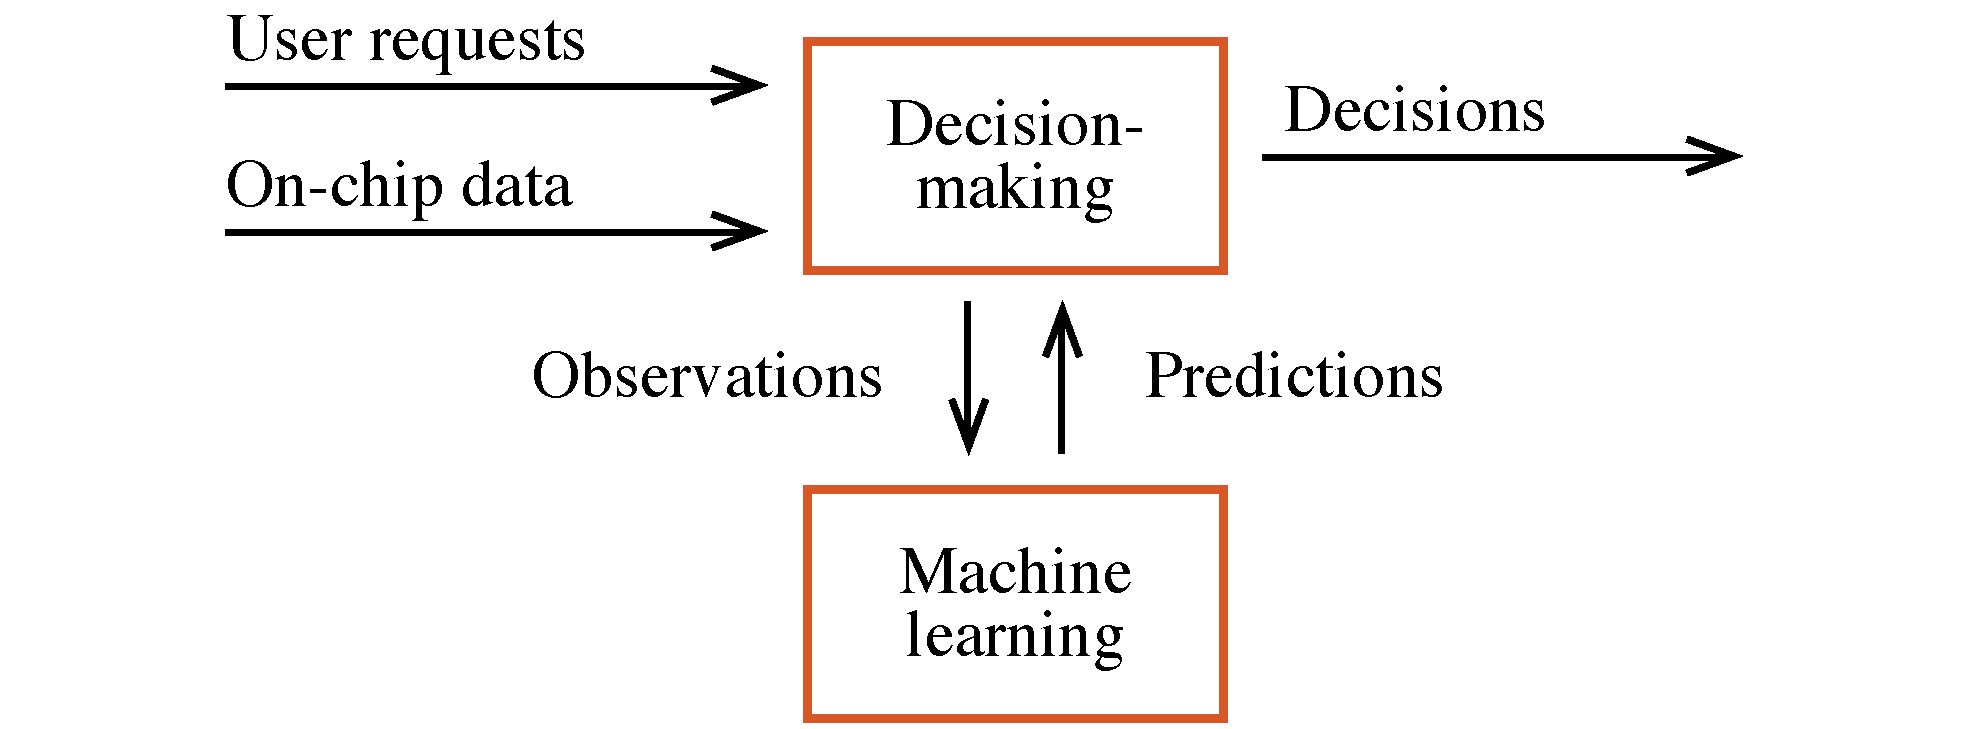
\includegraphics[width=1.0\columnwidth]{include/assets/figures/governor.pdf}

  \caption{A proactive governor of an electronic system. \emph{Observations}
  refers to the data used for learning. \emph{Predictions} refers to the data
  that the management strategy needs to know in advance in order to make
  proactive decisions.}

  \flab{governor}
\end{figure}

Power and temperature data should be available in a timely manner. Proactive
management strategies, which we shall also refer to as proactive governors, are
known to be more efficient than reactive ones since they aim at preventing
problems instead of recovering from the consequences of problems
\cite{coskun2008, chaudhry2015}, which, in particular, avoids slowing or
shutting down processing elements. Acting proactively requires peaking into the
future or, more formally, being able to forecast future behavior. Consequently,
the first step towards proactive power- and temperature-aware management---and,
hence, towards making electronic products more reliable and energy
efficient---is to predict power consumption and heat dissipation.

Predicting the future relies on learning from the past. This task is typically
accomplished by virtue of tools from statistics and adjacent fields such as
machine learning \cite{bishop2006}. In this case, a proactive governor contains
a learning component, which assimilates relevant on-chip data and makes
predictions. An illustration of this scenario is shown in \fref{governor}. To
give a concrete example, in \cite{coskun2008}, temperature forecasting is based
on an autoregressive moving-average model, enabling the development of an
efficient thermal management strategy for multiprocessor systems. The work in
\cite{kumar2010} aids runtime thermal management by developing an on-chip
temperature predictor based on artificial neural networks. The analysis and
mitigation of the impact of process variation undertaken in \cite{juan2014} are
facilitated by a linear-regression model trained on leakage measurements in
order to predict peak temperatures.

In the above, we have argued for the usage of learning-based techniques for the
management of electronic systems, and we have put emphasis on those techniques
that learn online, that is, at runtime on the chip, as they are capable of
adaptation. However, the present work is not concerned with the development of
any particular technique of this kind. Instead, the goal of our work is to
provide an infrastructure that facilitates the development of such techniques,
and this infrastructure addresses the following major concern.

\subsection{Data for Learning} \slab{simulation}
\begin{figure}
  \centering
  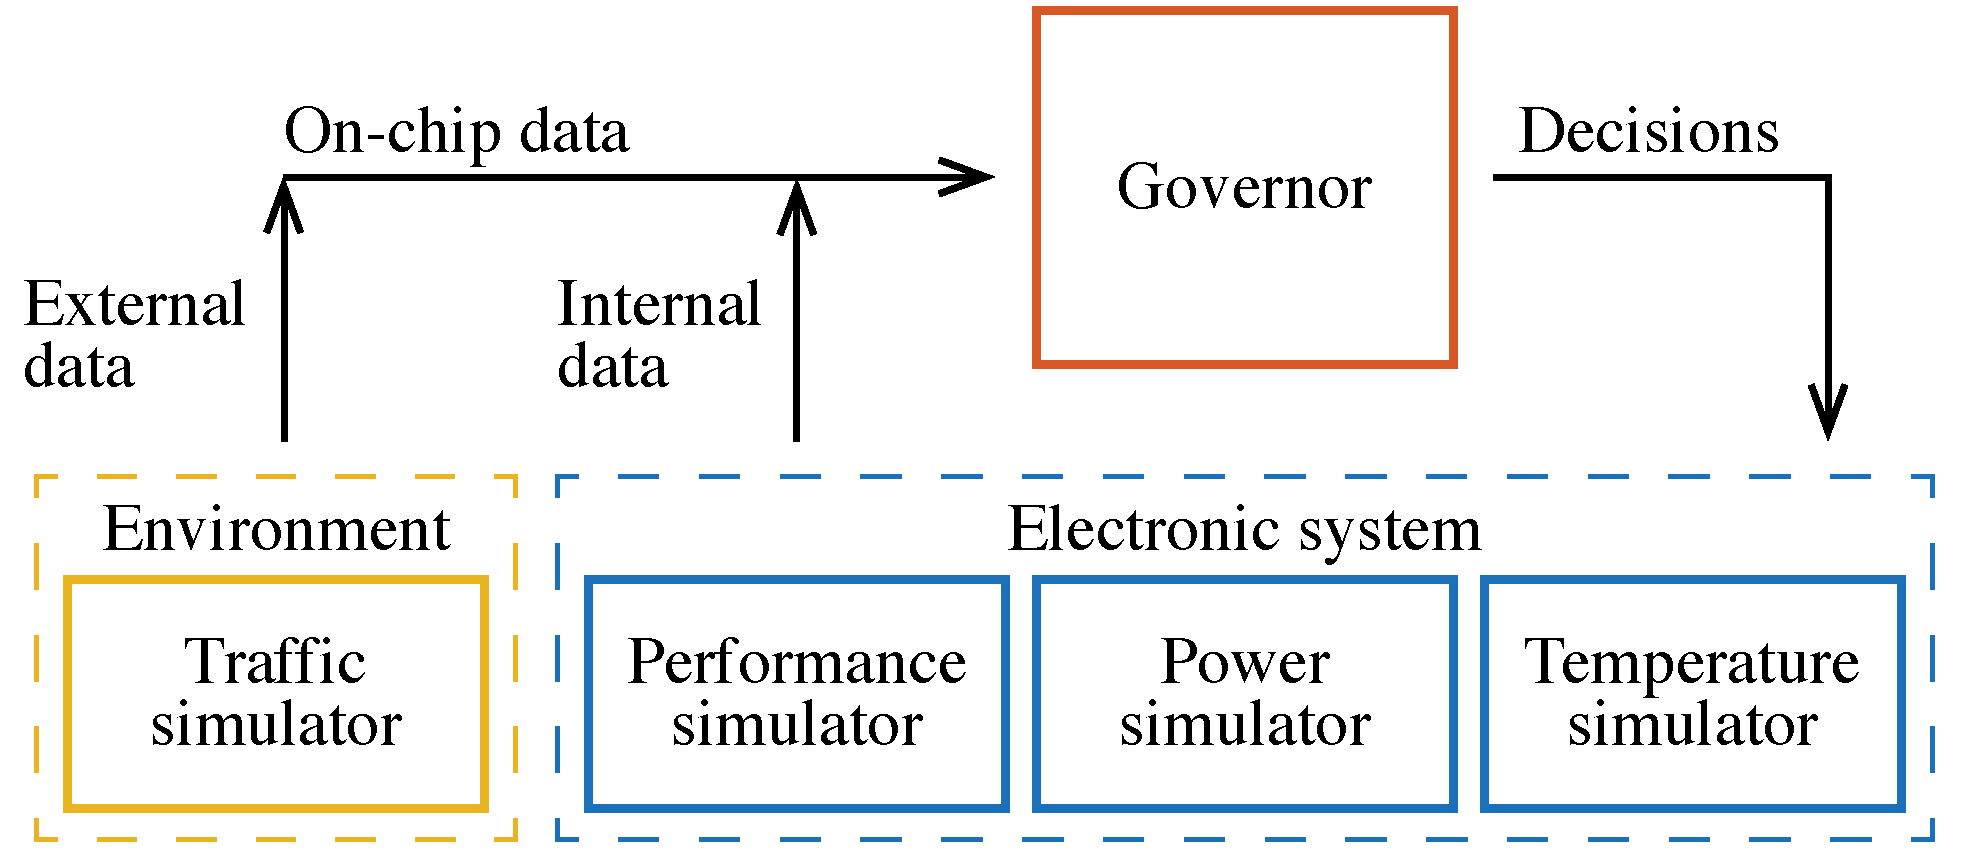
\includegraphics[width=1.0\columnwidth]{include/assets/figures/development.pdf}

  \caption{An experimental setup for developing management strategies
  (governors). \emph{Online data} refers to the data available on the chip
  regardless of their origin. The right dashed box should be understood at a
  single module, and the corresponding arrows should be treated accordingly.}

  \flab{development}
\end{figure}

Regardless of the learning tool utilized, the tool needs data to learn from.
Prior to a physical instantiation of the platform under consideration, all the
hope rests on the shoulders of computer models and simulators. The need for
simulators is not any lower even when an existing platform is concerned. The
platform might not be available to the interested party, or it might not be an
appropriate place for early experimentation and fluid exploration, which is
arguably the most common scenario in research. In such cases, computer
simulators are of great help, and their ubiquitous usage speaks to this
assertion. Therefore, a typical research environment used for developing a
governor of an electronic system is composed of a number of simulators,
providing data to and processing data from the governor. An illustration of such
an environment is given in \fref{development} wherein Governor is the one
depicted in \fref{governor}, and the purpose of the other modules will be made
clear later on.

Simulations can be undertaken on different levels, depending on the goal in
mind. In order to be useful for learning purposes, simulations should be
sufficiently detailed so that they capture well the traits of real systems.
Although detailed simulations (down to cycle accuracy) are practical for the
design of individual components, such simulations fall short when it comes to
complex systems. A modern multiprocessor system is reasonably complex, and it
might take days for a state-of-the-art simulator (not even cycle accurate) to
simulate a short, in wall-clock time, program running on such a system. This
scheme is not affordable for designing data-driven techniques as they require
many simulations with potentially large payloads.

The conclusion is that real data are rarely available, and simulation data are
prohibitively time consuming to obtain. Both are severely limiting from the
standpoint of a researcher trying to leverage the rich machinery of statistics
and machine learning. The need for alternative sources of high-quality data is
prominent, and providing such an alternative source is the very goal of this
work. More concretely, we are to build a highly responsive (time-wise) research
infrastructure, which is supposed to be used for the development of on-chip,
data-driven, power- and temperature-aware solutions for multiprocessor systems
instead of the one depicted in \fref{development}.


  \section{Prior Work}
  The present work is related to computer simulation. For our purposes, it is
sufficient to distinguish four types of simulation: traffic, performance, power,
and temperature, which are shown in \fref{development}. In this paper,
\emph{traffic} refers to a stream of jobs that lade the system with work, and
\emph{performance} to various performance metrics of the system such as the
numbers of executed instructions and read/write memory accesses.

Let us discuss traffic first. The Poisson process \cite{lifshits2014} is
arguably the most well-known model in this regard. However, the seminal work in
\cite{leland1994} and subsequent studies have shown that network traffic
exhibits fractal properties such as burstiness, self-similarity, and long-range
dependence. The Poisson process is unable to express any of these properties.
Another popular model is the fractional Gaussian noise \cite{lifshits2014},
which is a self-similar stochastic process. However, this process is suited for
modeling arrivals per unit of time but not for modeling arrival or inter-arrival
times, which are what is typically needed for simulation. Moreover, the noise
can take negative values and is a monofractal process, both of which are
unrealistic. The work in \cite{riedi1999} addresses the aforementioned concerns
by introducing a multifractal wavelet model for characterizing positive-valued
sequences with long-range-dependent correlations.

A performance simulator that we would like to highlight is Sniper
\cite{carlson2011}. Sniper is aimed at x86-based systems, and it has been
validated against Intel Core 2 and Nehalem architectures. The simulator works at
a higher level of abstraction than the one of cycle-accurate simulators, which
makes its simulation times more affordable. Regarding power simulation, a common
choice is the \sc{McPAT} framework \cite{li2009}. \sc{McPAT} is also capable of
estimating the areas occupied by processing elements, which is useful since this
information is essential for temperature simulation. Architecture-level
temperature simulation is arguably dominated by HotSpot \cite{skadron2004}. A
popular alternative is \sc{3D-ICE} \cite{sridhar2010}, which is particularly
focused on \sc{3D} structures.

The pipeline assembled from the aforementioned simulators is the one frequently
used in today's research (see the blue boxes in \fref{development}). However, as
we elaborate in \sref{introduction}, it is extremely time consuming and, hence,
is not suitable for learning purposes. In our experience, this is mainly due to
performance simulation and, to a lesser extent, power simulation. Temperature
simulation usually has a relatively small cost. These concerns are to be
discussed and illustrated in \sref{result}.

Our work makes the following major contribution. We present an efficient
toolchain for generating realistic power and temperature profiles of computer
systems in order to facilitate the development of intelligent data-driven
techniques for the analysis and management of such systems. The toolchain is
open source and publicly available online at \cite{sources}.
 \slab{literature}

  \begin{figure*}
  \centering
  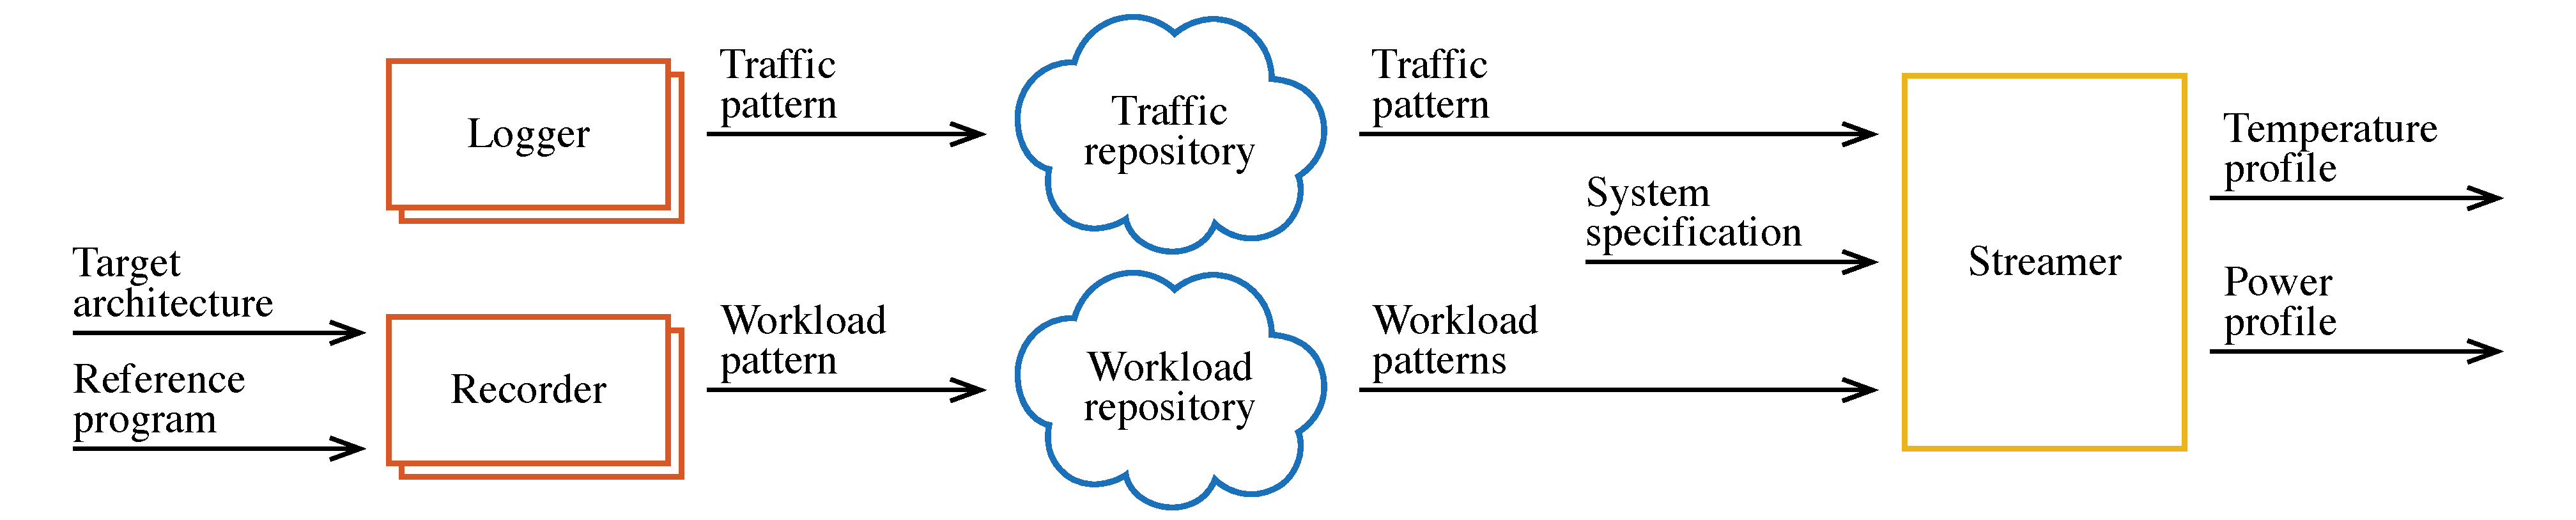
\includegraphics[width=1.0\textwidth]{include/assets/figures/methodology.pdf}
  \caption{
    Workflow of our methodology. The data-acquisition stage is to the left of
    the clouds, and the data-synthesis is to the right.
  }
  \flab{methodology}
  \vspace{-1em}
\end{figure*}

  \section{Our Contributions} \slab{contribution}
  Our work makes the following major contributions:

\begin{itemize}
  \item {\bfseries Contribution~1.} We draw attention to the need for developing
  substantially faster tools for generating data of electronic systems than
  those currently available in order to enable rapid exploration of advanced
  data-powered techniques for analysis and management of such systems.

  \item {\bfseries Contribution~2.} We present a methodology for generating
  realistic power and temperature profiles of multiprocessor systems,
  addressing the above concern.

  \item {\bfseries Contribution~3.} We develop and open-source a toolchain
  implementing the proposed methodology.
\end{itemize}

The first contribution is a topic penetrating the whole paper from the
introduction to the conclusion. The other two contributions are primarily
discussed starting from the next section onward. Let us now formalize the
problem that these two contributions are supposed to solve.


  \section{Problem Formulation} \slab{problem}
  Consider an in-design or in-production computer system. The system is composed
of a number of processing elements and is capable of performing a number of
operations. The system receives a stream of user requests or jobs, which it is
supposed to process. Each job implies a certain amount of work to be done and,
thus, a certain amount of power to be consumed and a certain amount of heat to
be dissipated.

Consider now a research project targeted at developing a resource manager for
the system under consideration. Since the importance of power and temperature is
well understood, the solution is required to take these two quantities into
account. Suppose further that the resource manager is to be based on a technique
that learns from the data available at runtime.

Our goal is to develop a toolchain for generating power and temperature profiles
of the system in order to provide the project with plenty of data to experiment
with. The generated profiles should preserve the particularities of job arrivals
and program executions that are present in real life, which is what makes the
subsequent learning meaningful. In addition, the generation process should be
substantially faster than traditional simulations, which is what makes the work
worth doing.


  \section{Methodology} \slab{methodology}
  In this section, we describe the workflow of the proposed methodology along with
the core ideas and models that the methodology is based on. Although our work is
closely related to simulation techniques, what we do is synthesis, not
simulation, which will become clear in the following subsections. An overview of
the methodology is depicted in \fref{methodology} and can be described as
follows. There are two major stages: data acquisition and data synthesis. The
leftmost modules in \fref{methodology} correspond to the data-acquisition stage,
and the rightmost module corresponds to the data-synthesis stage. The
data-acquisition stage collects and stores reference data while the
data-synthesis stage fetches these data and produces power and temperature
traces of the system. There are two types of reference data: traffic and
workload, which are referred to as patterns in the figure and in what follows.
As the names suggest, the two pieces of information characterize job arrivals
and job workloads, and they will be discussed further in \sref{traffic} and
\sref{workload}, respectively. In \sref{composition}, we shall explain how all
the pieces are combined into a coherent whole.

\subsection{Traffic} \slab{traffic}
\cite{leland1994}

In order to generate realistic steams of job arrivals, we have decided to use a
multifractal wavelet model \cite{riedi1999}, which was originally proposed in
the context of network traffic modeling. In vain with other studies
\cite{nikitovic2004}. We use a dataset published by Google \cite{google}. The
dataset contains usage data of a computational cluster over a month period (May
2011).


\subsection{Workload} \slab{workload}
In the previous subsection, we introduced our approach to generating streams of
arrivals; however, an arrival is only a time stamp without any information about
the actual workload. In this subsection, we describe how workload candidates are
obtained and utilized for substantiating job arrivals, which is depicted at the
bottom of \fref{methodology}. To begin with, workload candidates should conform
to a number of criteria. First, since we aim to produce realistic trace,
workloads should represent well the applications or services that the system in
question is supposed to provide to the user. Second, a workload should be fast
to evaluate, which, in our context, refers to obtaining the power consumption
over time of that workload.

Our workload modeling is based on full-system simulations of reference programs.
However, if we had incorporated such simulations into our workflow
\emph{directly}, we would have wound up with a configuration similar to the one
displayed in \fref{development}. This, of course, would have defeated the
purpose of our work since, as motivated in \sref{motivation}, detailed
simulations are too time consuming. Instead, we propose the use of high-level
recordings; this functionality corresponds to the modules labeled ``Recorder''
in \fref{methodology}. To elaborate, using an adequate simulator capable of
modeling the target architecture, we execute each reference program in isolation
and record certain information about this execution.\footnote{Such a technique
is similar in spirit to PinPlay \cite{patil2010}, which is a tool for recording
and replaying an execution of a program at the instruction level.} At a later
stage of our pipeline (see the Streamer module in \fref{methodology}), the
collected information is utilized in order to flesh out jobs upon their arrival,
and this stage requires no simulation. These recordings are building blocks:
they are combined to form complex workloads corresponding to multiple programs
running in parallel, which will be elaborated on in \sref{composition}.

From our experience, performance and power simulation takes by far the largest
expense in terms of time. Therefore, the information about a reference program's
execution that we propose to record is the power consumption of that execution.
This approach pushes the aforementioned expense to the data-acquisition stage
and eliminates it all together from the data-synthesis stage. To put it
differently, each recording is obtained via a one-time simulation at the
data-acquisition stage, and from there on the recording is reused as many times
as needed at the data-synthesis stage of our methodology. Since the actual data
generation, which takes place at the data-synthesis stage, is deliver from the
expensive simulations, it has a very low computational demand. This demand is
negligible compared to the one of the scenario depicted in \fref{development},
in which one undertakes performance and power simulations nonstop.

The power consumption of a program can be recorded differently; let us be more
specific about what we do. The first aspect to note is that we record power as a
function of time (assuming a certain sampling interval). Second, the dynamic and
static components of the power consumption are recorded separately in order to
get a better control over the subsequent composition (\sref{composition}).
Third, the power consumption is recorded for all processing elements that are
relevant to the subsequent study (for instance, cores and shared caches).

The result of the recording procedure is a repository of power traces
corresponding to real programs, which we refer to as workload patterns; see the
bottom cloud in \fref{methodology}. Full-system simulations obviously take time;
however, as mentioned previously, they should be done only once. Moreover, since
researchers tend to test their ideas using similar sets of benchmark
suites---for example, \sc{PARSEC} \cite{bienia2011} and \sc{SPEC CPU2006}
\cite{cpu2006} are popular choices---it is reasonable to create a common
repository of power patterns that will be populated and maintained online by the
research community.

Let us now turn to the question: How do we choose which workload pattern to use
for a particular arrival? We shall refer to this functionality as the workload
model. The input to this model is a stream of arrival times, and its output is a
stream of fully characterized jobs (time and work). The logic of the workload
model can be dependent on the input stream and thereby introduce
autocorrelations to the output stream, which allows for modeling, for instance,
periodic and/or coupled workloads. Since such aspects rely heavily on
domain-specific knowledge, we refrain from providing any particular dependency
model. The default option that is used in our toolchain (to be discussed in
\sref{toolchain}) for assigning workloads to job arrivals is drawing samples
from a uniform distribution over a set of workload patterns. This default
behavior can be adjusted for the problem at hand as needed.

To recapitulate, we have obtained a database of reference workloads and
discussed the formation of job streams from arrival streams. The patterns
correspond to executions of real programs and, thus, exhibit realistic traits.


\subsection{Composition} \slab{composition}
\begin{figure}
  \centering
  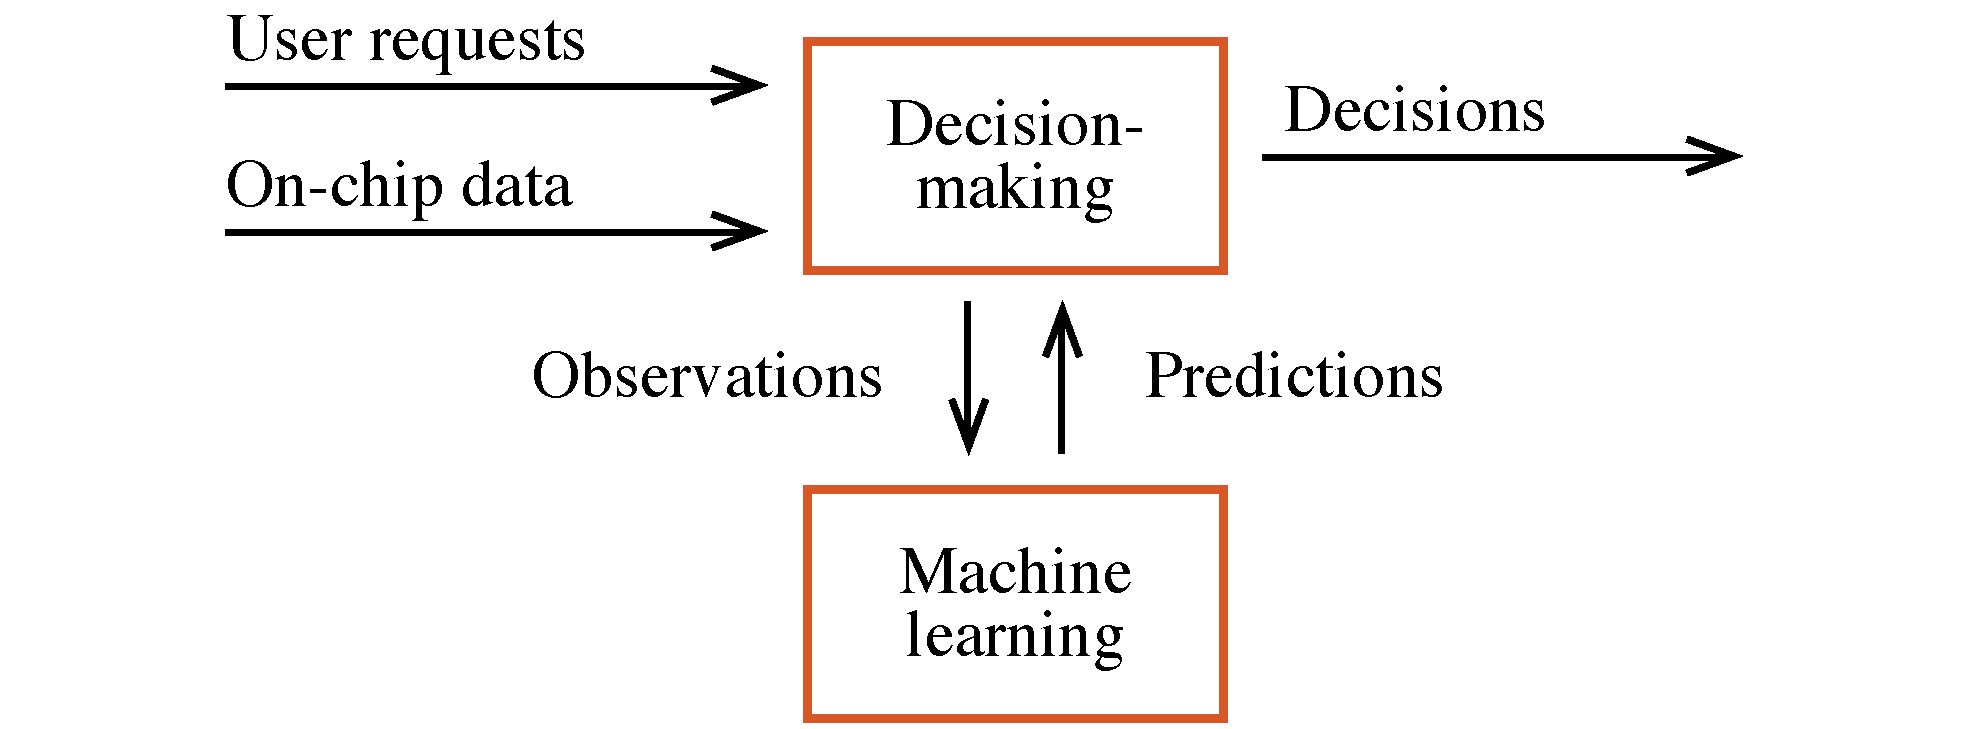
\includegraphics[width=1.0\columnwidth]{include/assets/figures/governor.pdf}

  \caption{A proactive governor of an electronic system. \emph{Observations}
  refers to the data used for learning. \emph{Predictions} refers to the data
  that the management strategy needs to know in advance in order to make
  proactive decisions.}

  \flab{governor}
\end{figure}

So far we have obtained two corresponding streams: arrival and workload. The two
streams merge into a new stream representing a sequence of concrete incoming
jobs or user requests, and this new stream needs to be processed, which is the
topic of this subsections. Here, \emph{processing} refers to progressively
building a schedule,\footnote{In this paper, mapping is assumed to be a part of
scheduling.} constructing a power profile, and computing the corresponding
temperature profile. In \fref{methodology}, this functionality resides in the
box labeled ``Streamer.''

As motivated in \sref{motivation}, a prominent use case of our methodology is
the development of management strategies. Therefore, the management core of the
system at hand is devised by the user, which is further detailed in
\sref{usage}. Hence, a scheduling policy is given, and it decides on a schedule.
Namely, each arrived job contains information about the computational resources
it needs, and the policy specifies when the job gets access to these resources.
Then we add accordingly the recorded (and potentially transformed) power pattern
of the job to the power profile of the system. A helpful analogy here might be
paving a road with rectangular bricks of different sizes. As the time goes by,
we feed the power profile to a temperature simulator and obtain a temperature
profile.

The power and temperature profiles are the final output of our methodology. The
key observation to be made is that no prohibitively expensive performance or
power simulations are involved in the data-synthesis stage. The time consumed by
the procedure delineated above is practically negligible.

At this point, we would like to draw attention to the following. It should be
clear that, by recording power directly, we make a trade-off, and making this
trade-off is necessary. Many details pertaining to programs' executions have
been discarded in order to gain speed. What has been baked into recordings
cannot be to altered at the data-synthesis stage in general. Consider, for
instance, a recording of a program that had two cores at its disposal. This
pattern cannot be used to replay the execution as if there was only one core.
Similarly, the recording cannot tell what would happen if the program could
leverage one additional core. Another limitation concerns resource sharing,
which is twofold. First, workload patterns obtained in isolation cannot used to
fabricate the interleaving of two programs (time sharing). Second, even if two
programs run on two different cores, they still can affect each other by
competing for such resources as shared L3 caches. Currently, the above concerns
can be addresses in our methodology only partially.


To summarize, the proposed methodology has been presented. The methodology is
composed of two stages. In the data-acquisition stage, reference arrival and
workload data are harvested. In the data-synthesis stage, the data are used to
generate a stream of jobs and subsequently compute a power and a temperature
profile. The produced data preserve the particularities of the reference data.
At the same time, the synthesis is fast as it bypasses expensive simulations.


  \section{Toolchain} \slab{toolchain}
  The toolchain has been implemented in the Rust programming language
\cite{rust}.\footnote{Rust is a systems programming developed by Mozilla
Research and thousands of independent contributors from all around the world.
Rust focuses on memory safety without garbage collection, concurrency without
data races, abstractions without overhead, and stability without stagnation.} It
consists of a number of programs, and the programs are composed of a number of
stand-alone packages. The toolchain also makes use of third-party software.
Regardless of the origin, each component of the toolchain is open source. The
code written by us is distributed under the \sc{MIT} license \cite{mit} and is
available at \cite{sources}. Feedback is welcome, and contribution will be very
much appreciated.

The main programs of our toolchain are called \recorder\ and \streamer, and we
shall describe them next.

\subsection{Recorder}
\begin{figure}
  \centering
  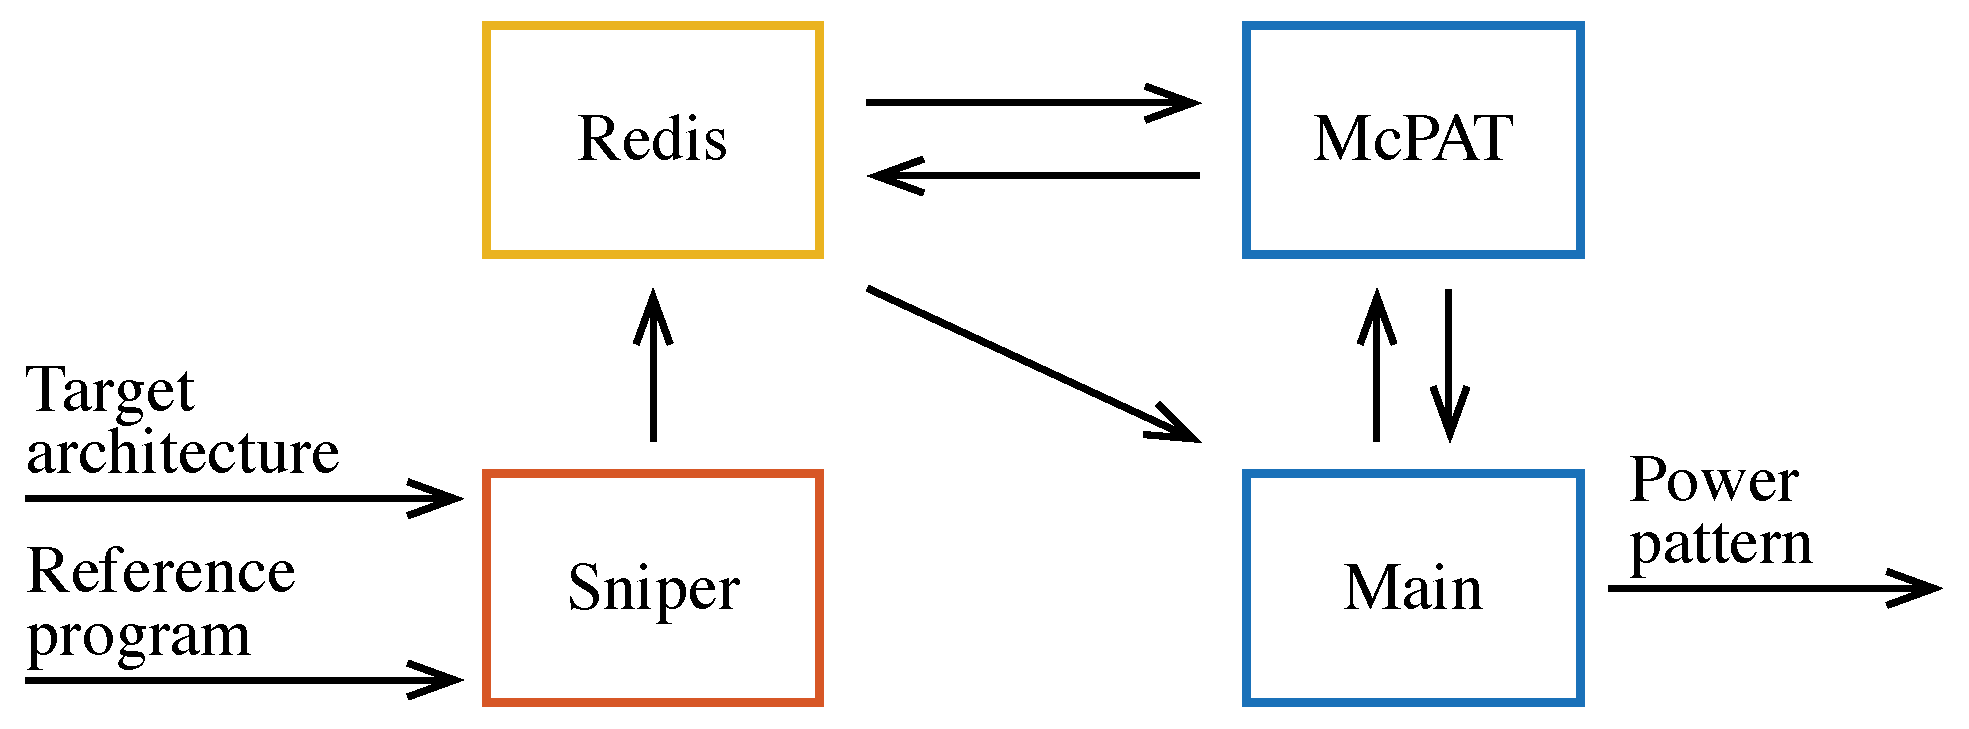
\includegraphics[width=1.0\columnwidth]{include/assets/figures/recorder.pdf}
  \caption{
    The recording infrastructure. The Recorder tool corresponds to the two blue
    boxes on the right-hand side of the figure.
  }
  \flab{recorder}
\end{figure}

\begin{table}
  \begin{threeparttable}
    \caption{Target architecture}
    \begin{tabular*}{\linewidth}{=L{70pt}l}
      \toprule
      Component    & Description \\
      \midrule
      Core         & 2660 MHz, 1.2 V \\
      L1-I/D cache & 32 KB, 4-way, LRU, private \\
      L2 cache     & 256 KB, 4-way, LRU, private \\
      L3 cache     & 8192 KB, 16-way, LRU, one per four cores \\
      \bottomrule
    \end{tabular*}
    \tlab{target}
    \begin{tablenotes}
      \item A detailed description of the target architecture can be found in
      the \texttt{nehalem.cfg} and \texttt{gainestown.cfg} configuration files
      of Sniper.
    \end{tablenotes}
  \end{threeparttable}
\end{table}
% vim: nowrap tw=0

As the name suggests, the purpose of \recorder\ is recording. More specifically,
the tool records reference workload patterns, which are needed as an input to
\streamer. The recording infrastructure is depicted in \fref{recorder}.

The performance simulator is Sniper \cite{carlson2011}.

The power simulator is \sc{McPAT} \cite{li2009}.

The key-value storage is Redis \cite{redis}.

The database is SQLite \cite{sqlite}.


\subsection{Streamer}
\begin{figure}
  \centering
  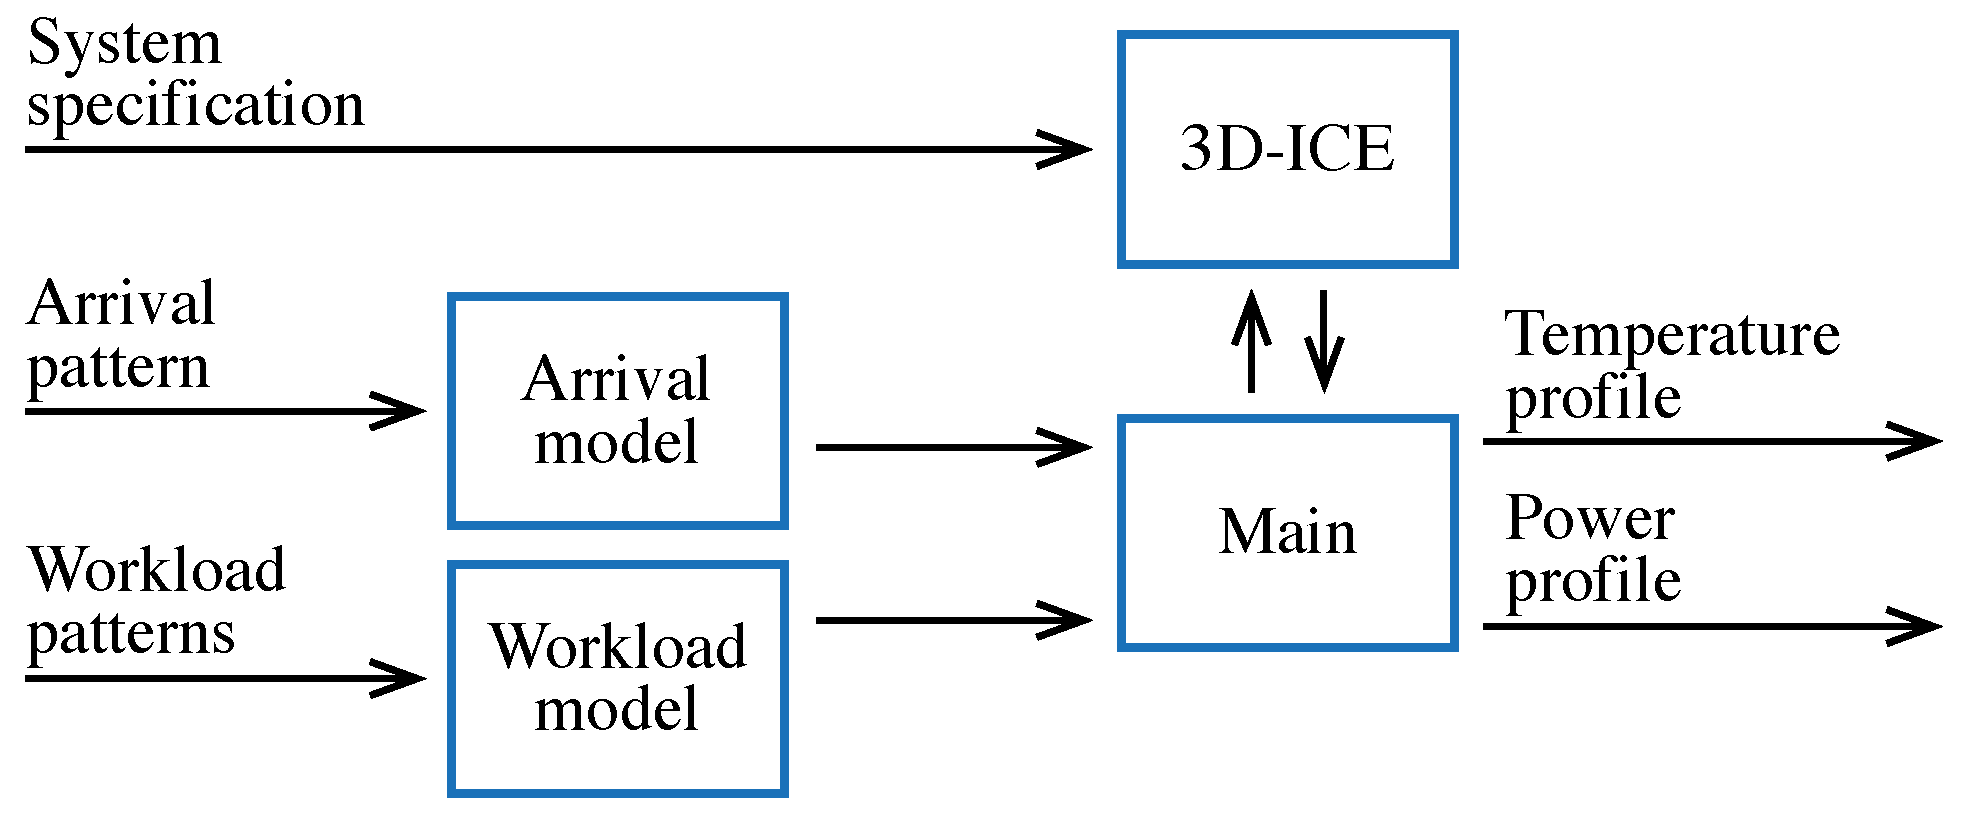
\includegraphics[width=1.0\columnwidth]{include/assets/figures/streamer.pdf}

  \caption{The Streamer tool. \emph{System specification} refers primarily to
  the information about the thermal package and floorplans of the platform,
  which are needed for temperature simulation. \emph{Job model} refers jointly
  to the traffic and workload models (\sref{traffic} and \sref{workload}).}

  \flab{streamer}
\end{figure}

The Streamer tool corresponds to the data-synthesis stage, which means that it
is responsible for synthesizing power and temperature data using reference data
as a material for the synthesis; see the module labeled ``Streamer'' in
\fref{methodology}. The structure of the tool is laid out in \fref{streamer}.

Given a traffic pattern and a set of workload patterns, Streamer proceeds as
follows. The traffic pattern is processed as it was described in \sref{traffic},
which results in an adequately configured multifractal wavelet model
\cite{riedi1999}. The model is then used to generate a stream of arrival times.
The arrival times are fleshed out using the workload patterns, which was
explained in \sref{workload}. The result is a stream of jobs, and the whole
operation is referred to as job modeling in \fref{streamer}. The rest follows
\sref{composition}. The job stream is handled by a scheduling policy; in
\fref{streamer}, this policy is a part of the Main module. As the incoming jobs
are being scheduled, the power profile of the system under consideration is
being constructed. The power profile is piped into a temperature simulator (to
be discussed below), which delivers a temperature profile. The continuity of the
process is worth noting: just as with arrival times and jobs, power and
temperature can be viewed as streams of data. The synthesized data (power and
temperature) can be fed back to the scheduler and/or stored for later usage. In
the latter case, similar to reference data, the output is an SQLite database.

Let us now outline how temperature simulation is undertaken inside Streamer. The
simulation is based on the popular thermal \sc{RC} model. In this paradigm, a
so-called thermal \sc{RC} circuit representing the system at hand is constructed
and then used to analyze the thermal behavior of the system. The analysis boils
down to solving a system of differential equations, which can be done using
different integration techniques. In our case, the solution is based on a solver
leveraging exponential integrators \cite{hochbruck2010, ukhov2014}. The
construction of thermal circuits is outsourced to either HotSpot
\cite{skadron2004} or \sc{3D-ICE} \cite{sridhar2010} (see \fref{streamer}). Both
simulators are based on the thermal \sc{RC} model, and we extract the circuits
that they build, which results in a unified interface for working with the two
alternatives.

To summarize this subsection, the Streamer tool produces streams of power and
temperature data, and this procedure closely follows the ideas presented in
\sref{methodology}. Our temperature simulation is based on the thermal \sc{RC}
model, in which thermal circuits are constructed by either HotSpot or
\sc{3D-ICE}.



  \section{Experimental Results} \slab{result}
  This section illustrates the performance of the toolchain presented in
\sref{toolchain}. All the experiments reported below are conducted on a
\sc{GNU}/Linux machine equipped with 16 \sc{CPU}s Intel Xeon E5520 2.27~\sc{GH}z
and 24~\sc{GB} of \sc{RAM}.

In order to obtain real-life traffic patterns for our experiments, we use a
large data set published by Google in 2011 \cite{reiss2011}. The data set
contains usage data of a computer cluster over a month period. We have
downloaded the table tracking the life cycle of the jobs submitted to the
cluster and extracted the time stamps of the first event related to each job. As
a result, there are around 670\,000 arrival times available, which we use for
fitting the traffic model as it is described in \sref{traffic}.

A set of workload patters is obtained by simulating and recording (via our
infrastructure shown in \fref{recorder}) the programs from the popular
\sc{PARSEC} \cite{bienia2011} and \sc{SPEC CPU2006} \cite{cpu2006} benchmark
suites; the former contains 13 programs, and the latter 29 programs. The
architecture used in these simulations is Intel's Nehalem-based Gainestown
series; Sniper is shipped with a configuration for this architecture
(\tt{nehalem.cfg} and \tt{gainestown.cfg}), and we used it without any changes.

All the reference data that we have collected and processed to make them
suitable for our toolchain are available at \cite{sources}.

\subsection{Recording}
\setlength{\tabcolsep}{4pt}
\begin{table}
  \begin{threeparttable}
    \caption{Recording (the \sc{PARSEC} benchmark suite)}
    \begin{tabular*}{\linewidth}{=L{43pt}-R{24pt}-R{28pt}-R{24pt}-R{24pt}-R{28pt}-R{24pt}}
      \toprule
      & \multicolumn{3}{c}{Recording time (hours)} & \multicolumn{3}{c}{Simulated time (seconds)} \\
      Program       & Small & Medium & Large & Small & Medium & Large \\
      \cmidrule( r){1-1}
      \cmidrule(l ){2-4}
      \cmidrule(l ){5-7}
      blackscholes  &  0.18 &  0.74 &  3.00 & 0.07 & 0.28 &  1.13 \\
      bodytrack     &  0.51 &  2.00 &  7.36 & 0.17 & 0.70 &  2.71 \\
      canneal       &  0.61 &  1.74 &  4.04 & 0.18 & 0.67 &  1.72 \\
      dedup         &  1.35 &  3.48 & 17.20 & 1.97 & 2.85 & 10.75 \\
      facesim       & 12.68 & 13.18 & 15.48 & 7.84 & 7.93 &  7.87 \\
      ferret        &  0.83 &  2.65 & 12.15 & 0.40 & 1.06 &  4.59 \\
      fluidanimate  &  0.78 &  2.18 &  6.90 & 0.53 & 1.32 &  4.11 \\
      freqmine      &  1.24 &  4.87 & 18.04 & 0.67 & 2.63 &  9.21 \\
      raytrace      &  4.22 &  5.69 & 10.08 & 0.24 & 0.63 &  1.51 \\
      streamcluster &  0.74 &  2.88 & 15.71 & 0.34 & 1.40 & 10.68 \\
      swaptions     &  0.59 &  2.33 &  9.05 & 0.23 & 0.91 &  3.64 \\
      vips          &  1.57 &  4.89 & 14.47 & 0.53 & 1.59 &  4.39 \\
      x264          &  0.49 &  2.59 &  8.61 & 0.17 & 0.99 &  3.09 \\
      \bottomrule
    \end{tabular*}
    \tlab{recording}
    \begin{tablenotes}
      \item \emph{Small}, \emph{medium}, and \emph{large} signify the input size
      of the programs.
    \end{tablenotes}
  \end{threeparttable}
\end{table}
% vim: nowrap tw=0

In the above, we outlined how the reference workload data were harvested using
the Recorder tool and the infrastructure around it, which were discussed in
\sref{recorder} and are displayed in \fref{recorder}. Now we show and elaborate
on the performance characteristics of this recording process.

The benchmark suite that we shall look at is \sc{PARSEC}. Our findings are
summarized in \tref{recording}. \sc{PARSEC} provides several choices of inputs
to the programs, and we recorded each program with three different inputs,
namely, with the ones classified as small, medium, and large. There are two
types of information shown in \tref{recording}: recording time (in hours), which
is the time that was taken to simulate and record the programs, and simulated
time (in seconds), which is the time that the programs would have taken in real
life. The sampling interval used in all experiments is one millisecond.

Each input class was recorded in a single batch: all 13 programs were simulated
simultaneously using 13 Sniper processes, which was explained and motivated in
\sref{streamer}. Consequently, the total recording time with respect to each
batch is dictated by the program that took the most time to finish. For small
and medium inputs, this program was \texttt{facesim}, which took approximately
13 hours in both cases. The simulated times of \texttt{facesim} indicate that
\sc{PARSEC} actually has only one input size for this particular program.
Regarding large inputs, \texttt{freqmine} finished last; more concretely, the
program took 18 hours. As an aside for the curious reader, the simulated and
recording times of \sc{SPEC CPU2006} (not shown) were an order of magnitude
larger than the ones of \sc{PARSEC}.

It can be seen in \tref{recording} that the throughput in terms of simulated
time is (expectedly) low: roughly speaking, two--three hours of recording time
amounts to one second of simulated time. However, it is important to realize
that these are one-time expenses in our methodology; the situation would be
drastically worse if one had to perform such simulations all the time (see
\sref{workload}). Another important aspect to note is that the observed
recording times have been substantially reduced by the choice of performance
simulator---Sniper is based on novel simulation ideas \cite{carlson2011}---and
the parallelization strategy and caching mechanism described in \sref{streamer}.


\subsection{Streaming}
\setlength{\tabcolsep}{4pt}
\begin{table}
  \begin{threeparttable}
    \caption{Streaming}
    \begin{tabular*}{\linewidth}{=L{50pt}-R{40pt}-R{40pt}-R{40pt}-R{40pt}}
      \toprule
      \multirow{2}{*}{\parbox{50pt}{Synthesized time (seconds)}} & \multicolumn{4}{c}{Synthesis time (seconds)} \\
      & $4 + 1$ & $8 + 2$ & $16 + 4$ & $32 + 8$ \\
      \cmidrule( r){1-1}
      \cmidrule(l ){2-5}
         10 &   0.24 &   0.40 &   0.67 &   1.13 \\
        100 &   2.11 &   3.66 &   6.18 &  10.19 \\
       1000 &  20.59 &  37.47 &  64.58 & 104.00 \\
      10000 & 214.98 & 394.84 & 598.89 & 984.59 \\
      \bottomrule
    \end{tabular*}
    \tlab{streaming}
    \begin{tablenotes}
      \item ``$M + N$'' stands for $M$ cores and $N$ L3 caches. Each four cores
        have a shared L3 cache; therefore, it holds that $N = M / 4$.
    \end{tablenotes}
  \end{threeparttable}
\end{table}
% vim: nowrap tw=0

Let us turn to the Streaming tool, which corresponds to the data-synthesis stage
of the methodology (see \fref{methodology}). Streamer was introduced in
\sref{streamer} and is depicted in \fref{streamer}. Our objective in this
subsection is to study the scalability of the tool as measured by synthesis
time, which is the time that is needed for the tool to synthesize power and
temperature profiles under certain conditions or requirements.

Before we proceed, let us reiterate that, as far as Streamer is concerned, the
expense of performance and power simulation is essentially zero as the tool
works with precomputed power data (power patterns). The most time-consuming part
of Streamer is temperature simulation, which is actually negligibly small (see
below) compared to the time shown in \tref{recording}.

The preformed experiments are consolidated in \tref{streaming}. We report
synthesis time along two dimensions: synthesized time (rows) and platform size
(columns). The former is analogous to simulated time, and the latter represents
different platforms as follows. Each considered platform is composed of a number
of cores, and there is an L3 cache for every four cores; both cores and caches
are referred to as processing elements. Platform size is then defined as the
number of processing elements, and it is denoted by ``$M + N$'' in
\tref{streaming} where $M$ and $N$ are the numbers of cores and caches,
respectively.\footnote{The specifications of the considered platforms are a part
of our supplementary materials available at \cite{sources}.}

Unlike the throughput of simulation (discussed in the previous subsection), the
throughput of synthesis in terms of synthesized time is very high, which is well
supported by \tref{streaming}. For instance, it takes Streamer around a minute
to produce power and temperature data that are worth around 17 minutes of
runtime of a multiprocessor system with 16 cores, which would be practically
infeasible to achieve with full-fledged simulations (refer to \tref{recording}).

Another observation made from \tref{streaming} is that synthesis time scales
linearly with respect to the length of the time span being synthesized
(synthesized time), and the same can be concluded regarding platform size. The
growth with respect to platform size is due to the increasing complexity of the
underlaying thermal \sc{RC} circuit used for temperature simulation; thermal
circuits were elaborated on in \sref{streamer}.


To summarize, the results reported in \tref{recording} motivate our work and
communicate well the message of this paper: the speed of the state-of-the-art
simulators is severely onerous for the purpose of experimenting with data-driven
techniques. The core problem is that such techniques typically require lots of
data (long execution traces); moreover, these data might need to be recalculated
each time a parameter changes (for instance, the parameterization of the
scheduling policy). The results in \tref{streaming} show that the proposed
approach can efficiently tackle this problem by taking the data burden away and,
hence, making it easier to experiment with data-driven techniques.


  \section{Conclusion} \slab{conclusion}
  In this paper, we emphasized the need for developing tools for studying
electronic systems with data-driven applications in mind. We argued that the
techniques capitalizing on learning from data have special requirements, and
that the state-of-the-art simulators are unable to fulfill them due to
prohibitively large simulation times. Acknowledging the importance of power and
temperature for the design of multiprocessor systems, we developed a methodology
for fast generation of synthetic power and temperature traces that preserve the
idiosyncrasies of their real-life counterparts. Last but not least, we
implemented a toolchain that embodies the presented approach, which was
subsequently assessed and shown to be extremely fast.


  \begingroup
    \linespread{0.9}
    \bibliographystyle{IEEEtran}
    \bibliography{IEEEabrv,include/bibliography}
  \endgroup
\end{document}
